% ||||||||||||||||||||||||||||||||||||||||||||||
% Capitulo de análise dos resultados
% ||||||||||||||||||||||||||||||||||||||||||||||
\chapter{Análise dos Resultados}



%%%%%%%%%%%%%%%%%%%%%%%%%%%%%%%%%%%
\subsection{Método de Sintonia via Método de Ziegler-Nichol em Malha fechada}

\begin{figure}[H]
  \caption{Respostas ao Degrau com sintonia via Método de Ziegler-Nichol em Malha fechada}
  \begin{center}
      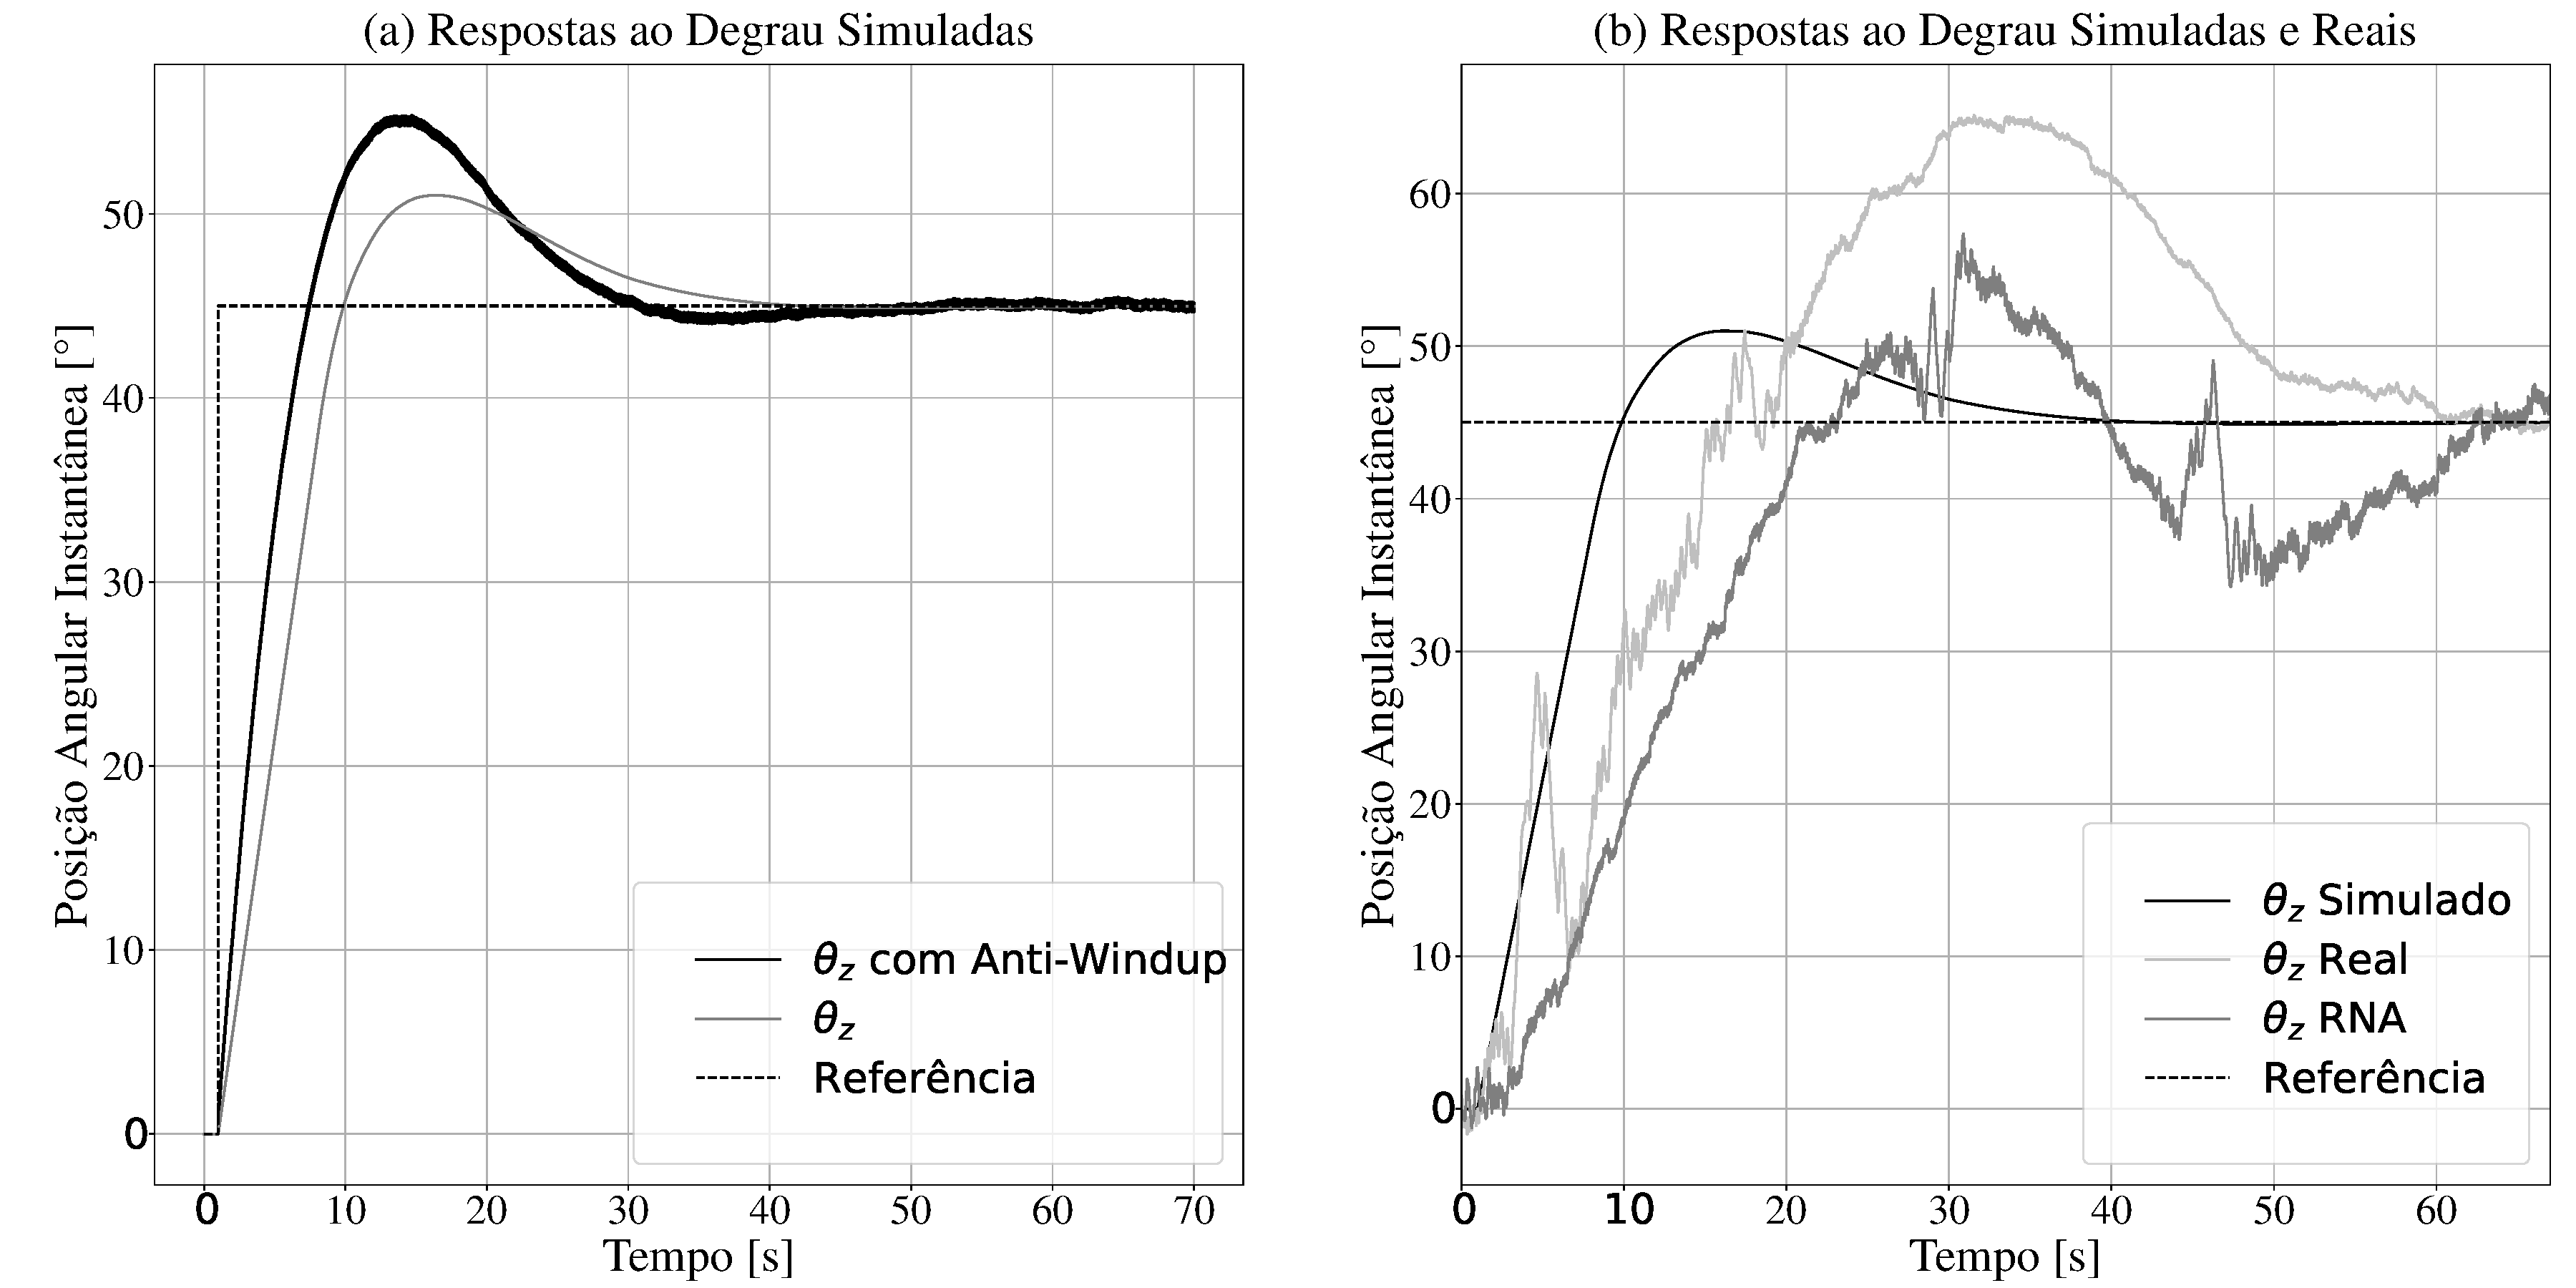
\includegraphics[scale=0.4]{resultados/img/pid_result}
  \end{center}
  \fonte{Elaborado pelo Autor.} 
  \label{fig:mpu6050_analisys}
\end{figure}

%%%%%%%%%%%%%%%%%%%%%%%%%%%%%%%%%%%
\subsection{Método de Sintonia Automático via Relé Com Histerese}

\begin{figure}[H]
  \caption{Respostas ao Degrau com Sintonia via Método do Relé}
  \begin{center}
      \includegraphics[scale=0.4]{resultados/img/white}
  \end{center}
  \fonte{Elaborado pelo Autor.} 
  \label{fig:mpu6050_analisys}
\end{figure}


%%%%%%%%%%%%%%%%%%%%%%%%%%%%%%%%%%%

\subsection{Método de Sintonia Automático usando Redes Neurais e Regrão Não-Linear Robusta}

\subsubsection{Treinamento da Rede Neural}

\begin{figure}[H]
  \caption{Saída da Rede Neural Treinada e o sinal Real}
  \begin{center}
      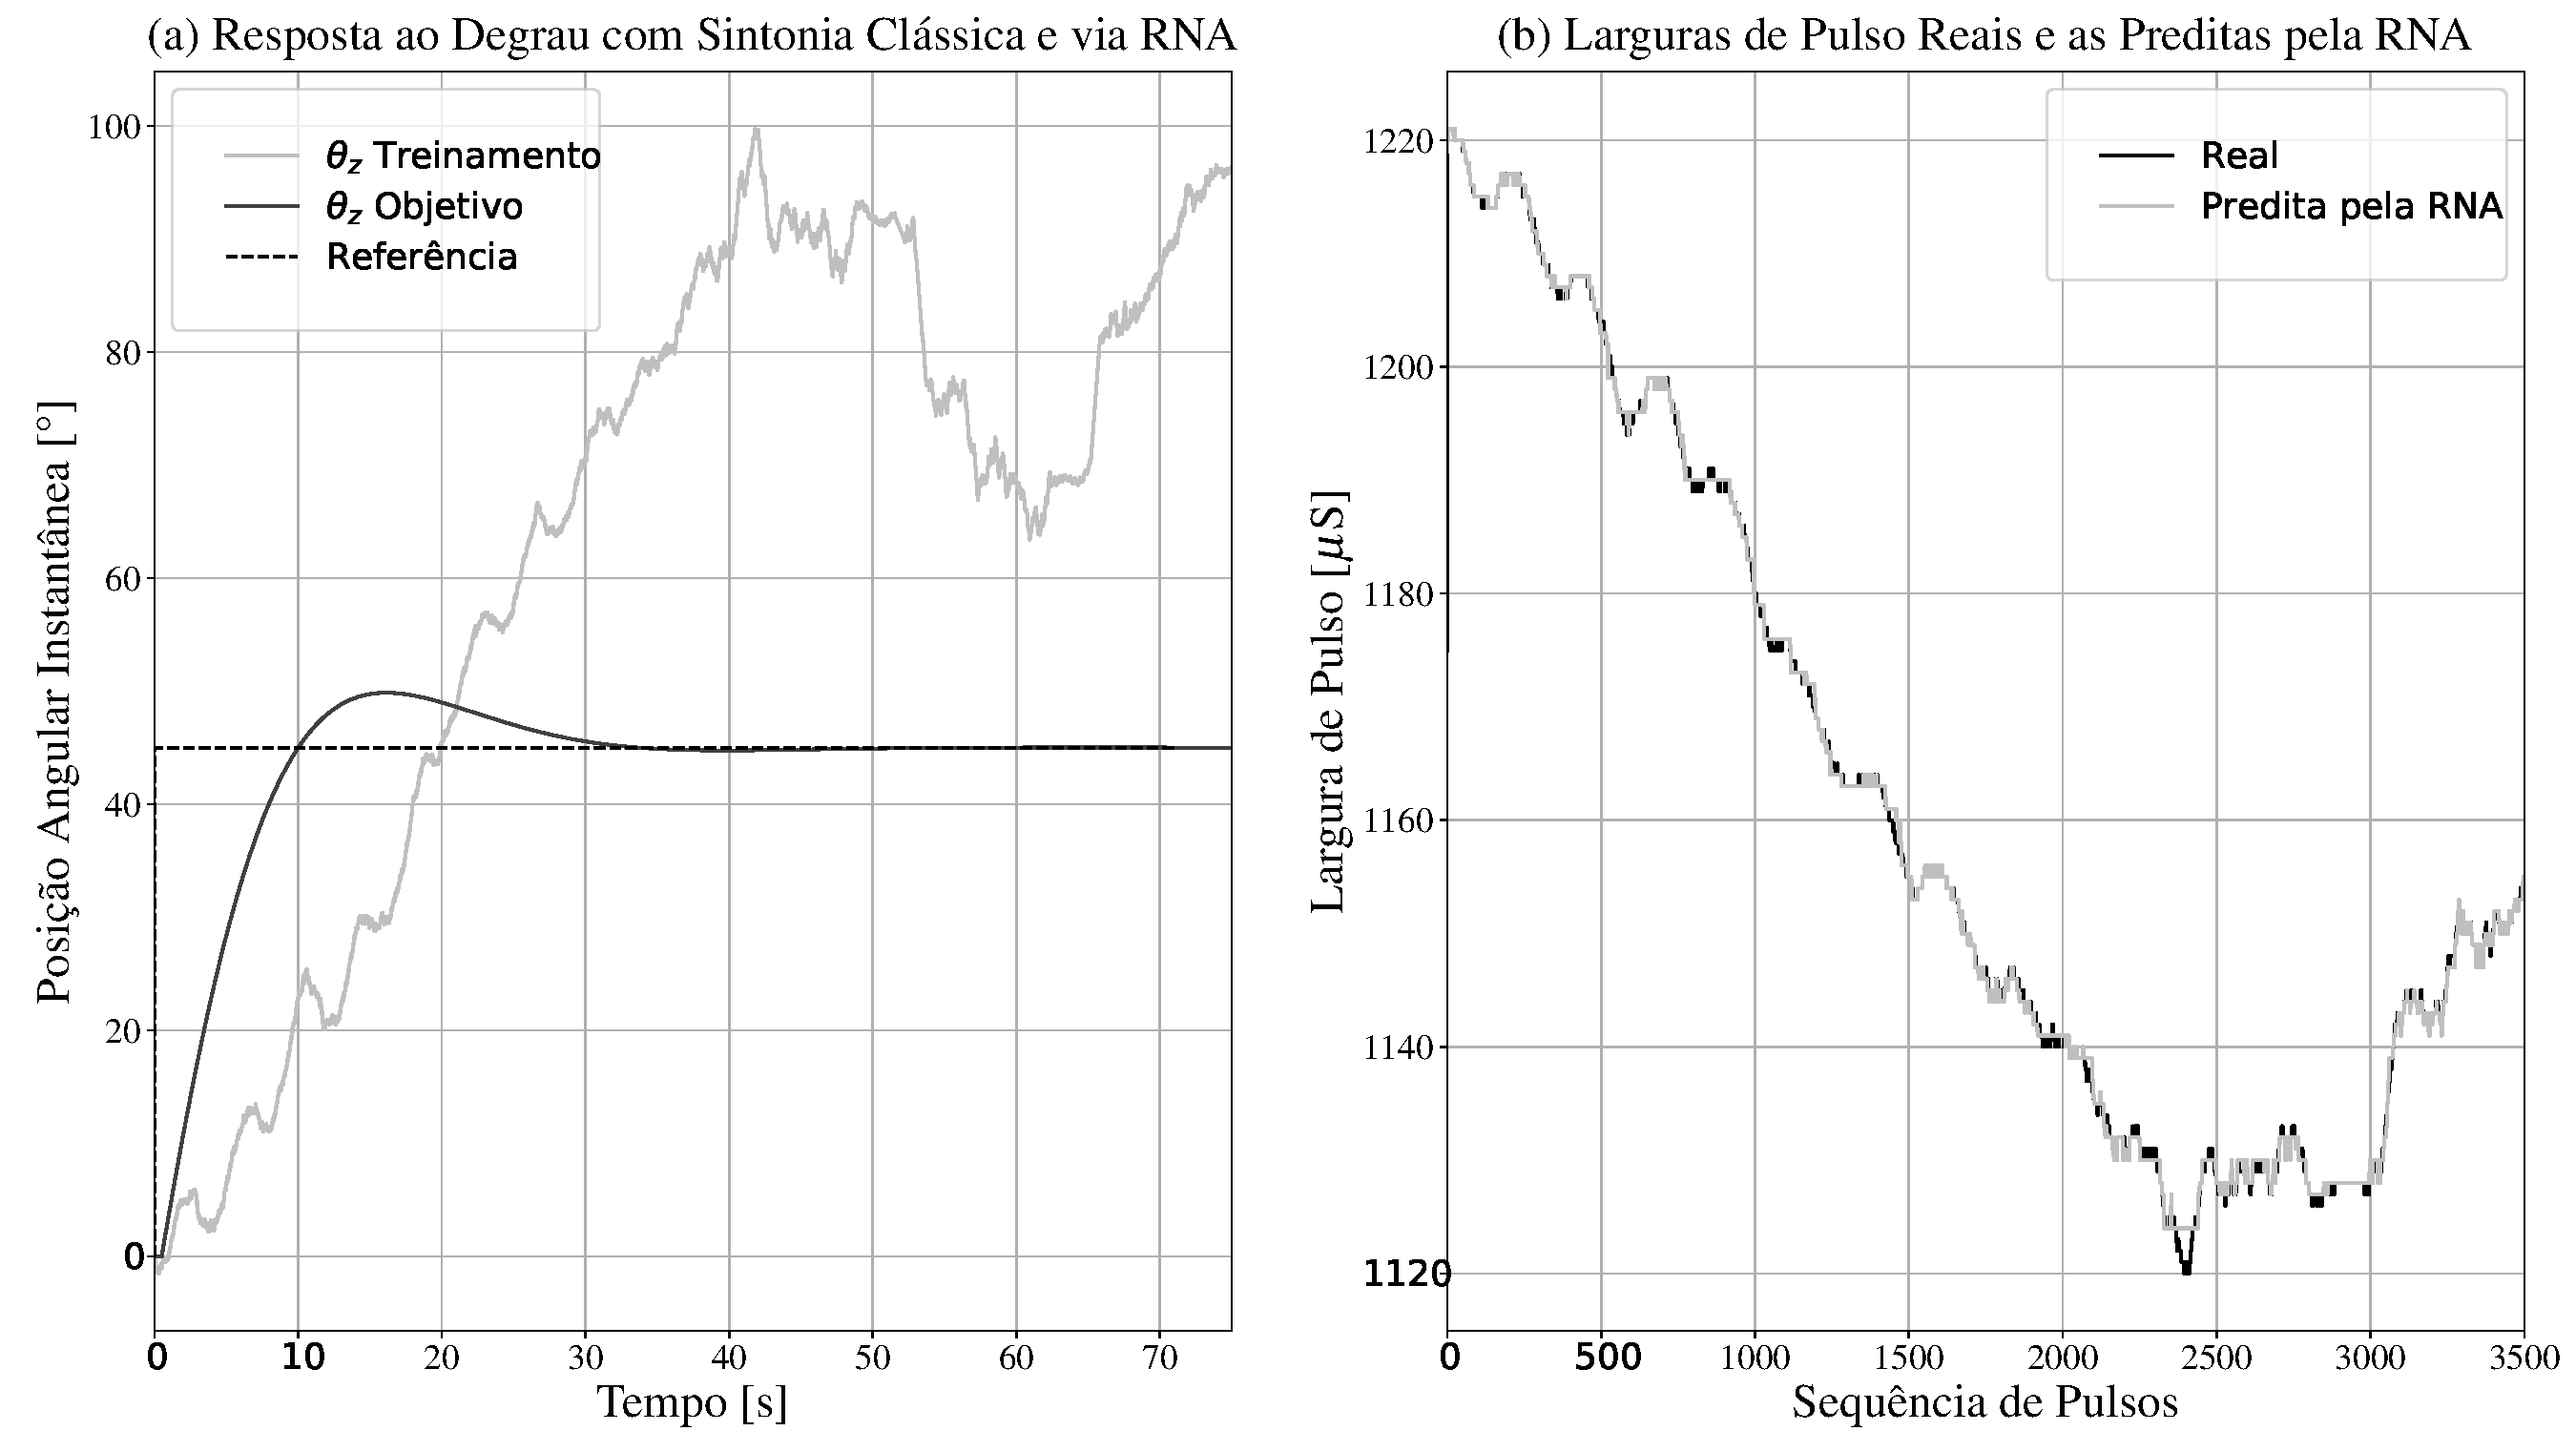
\includegraphics[scale=0.35]{resultados/img/neural_output}
  \end{center}
  \fonte{Elaborado pelo Autor.} 
  \label{fig:mpu6050_analisys}
\end{figure}

\begin{figure}[H]
  \caption{Respostas ao Degrau com Sintonia via Rede Neural e Regressão Não-Linear}
  \begin{center}
      \includegraphics[scale=0.4]{resultados/img/white}
  \end{center}
  \fonte{Elaborado pelo Autor.} 
  \label{fig:mpu6050_analisys}
\end{figure}

